Consider the table of differences of binomial coefficients and iterated rascal numbers one more time
as there is another pattern we can spot.
\begin{figure}[H]
    \centering
    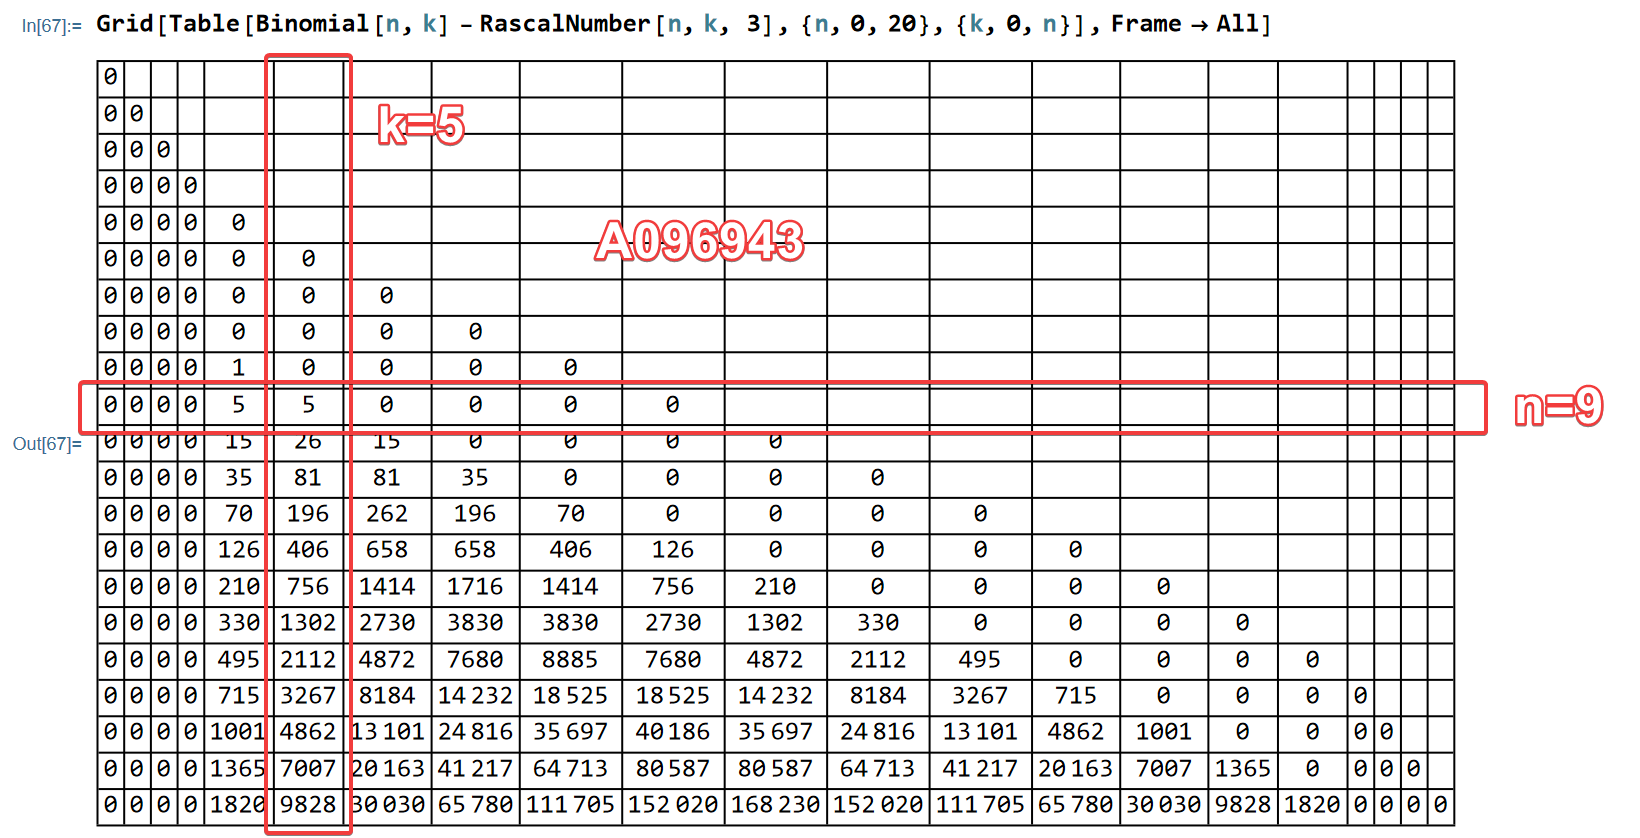
\includegraphics[width=1\textwidth]{img/03_Difference_Binomial_Rascal_i_3_OneQBinomialCoefficients}
    ~\caption{Difference $\binom{n}{k}-\rascalNumber{n}{k}{3}$.
    Highlighted column is $(1,5)$-binomial coefficient $\oneQBinomial{n}{k}{5}$.
    Sequence \href{https://oeis.org/A096943}{\texttt{A096943}} in the OEIS~\cite{sloane2004sixth}.}
    \label{fig:difference-qbinomial-rascal-i-3}
\end{figure}
The $(1,q)$-binomial coefficients $\oneQBinomial{n}{k}{q}$ are special kind of binomial coefficients defined by
\begin{definition}
    $(1,q)$-Binomial coefficient
    \begin{equation}
        \oneQBinomial{n}{k}{q} =
        \begin{cases}
            q & \mathrm{if} \; k=0, n=0 \\
            1 & \mathrm{if} \; k=0 \\
            0 & \mathrm{if} \; k > n \\
            \oneQBinomial{n-1}{k}{q} + \oneQBinomial{n-1}{k-1}{q}
        \end{cases}\label{eq:qbinomial-definition}
    \end{equation}
\end{definition}
Indeed, the relation shown in Figure~\eqref{fig:difference-qbinomial-rascal-i-3} is true for every $i$,
so that it establishes a relation between $(1,q)$-binomial coefficients and iterated rascal numbers.
\begin{proposition} (Relation between iterated rascal numbers and $(1,q)$-binomial coefficients.)
    For every $i\geq0$
    \label{prop:row-column-difference-qbinomial}
    \begin{align*}
        \binom{2i+3+j}{i+2} - \rascalNumber{2i+3+j}{i+2}{i} = \oneQBinomial{i+2+j}{i+2}{i+2}
    \end{align*}
\end{proposition}
Taking $t=i+2$ in~\eqref{prop:row-column-difference-qbinomial} yields
\begin{align*}
    \binom{2t-1+j}{t} - \rascalNumber{2t-1+j}{t}{t-2} = \oneQBinomial{t+j}{t}{t}
\end{align*}
In particular,
\begin{itemize}
    \item Having $i=1$ proposition~\eqref{prop:row-column-difference-qbinomial}
    gives the OEIS sequence \href{https://oeis.org/A006503}{\texttt{A006503}}~\cite{sloane1995n}
    such that third column of $(1,3)$-Pascal triangle
    \href{https://oeis.org/A095660}{\texttt{A095660}}~\cite{sloane2004pascal13}.
    \item Having $i=3$ proposition~\eqref{prop:row-column-difference-qbinomial}
    gives the OEIS sequence \href{https://oeis.org/A096943}{\texttt{A096943}}~\cite{sloane2004sixth}
    such that third column of $(1,5)$-Pascal triangle
    \href{https://oeis.org/A096940}{\texttt{A096940}}~\cite{sloane2004pascal}.
    \item Having $i=5$, the proposition~\eqref{prop:row-column-difference-qbinomial} yields
    the OEIS sequence \href{https://oeis.org/A097297}{\texttt{A097297}}~\cite{sloane2004seventh}
    such that seventh column of $(1,6)$-Pascal triangle
    \href{https://oeis.org/A096956}{\texttt{A096956}}~\cite{sloane2004pascal16}.
    \item Having $i=2$ and $k=4$: $\binom{n}{k} - \rascalNumber{n}{k}{i}$ gives
    Fifth column $(m=4)$ of $(1,4)$-Pascal triangle \url{https://oeis.org/A095667}
    \item Having $i=2$ and $k=3$: $\binom{n}{k} - \rascalNumber{n}{k}{i}$ gives
    Tetrahedral (or triangular pyramidal) numbers: $a(n) = C(n+2,3) = n*(n+1)*(n+2)/6$.
    \url{https://oeis.org/A000292}
    \item Having $i=1$ and $k=2$: $\binom{n}{k} - \rascalNumber{n}{k}{i}$ gives
    Triangular numbers: $a(n) = binomial(n+1,2) = n*(n+1)/2 = 0 + 1 + 2 + \dots + n$
    \url{https://oeis.org/A000217}
    \item Having $i=0$ and $k=3$: $\binom{n}{k} - \rascalNumber{n}{k}{i}$ gives
    Fourth column (r=3) of FS(3) staircase array.
    \url{https://oeis.org/A062748}
    \item Having $i=0$ and $k=6$: $\binom{n}{k} - \rascalNumber{n}{k}{i}$ gives
    $a(n) = binomial(n,6)-1$.
    \url{https://oeis.org/A124089}
    \item Having $i=0$ and $k=7$: $\binom{n}{k} - \rascalNumber{n}{k}{i}$ gives
    $a(n) = binomial(n,7)-1$.
    \url{https://oeis.org/A124090}
\end{itemize}
